\documentclass[
    11pt,
    spanish,
	a4paper
]{article}
\usepackage[utf8]{inputenc}
\usepackage[spanish]{babel}
\usepackage{graphicx}
\usepackage{authoraftertitle}
\usepackage{float}
\usepackage{caption}
\captionsetup[table]{labelformat=empty}

\def\doctype{TRABAJO PRÁCTICO FINAL}
\title{Oxímetro de pulso}
\author{Gonzalo Nahuel Vaca}

\begin{document}

\makeatletter
\begin{titlepage}
	\begin{center}
		\vspace*{1cm}
		
		\Huge
		\textbf{\doctype}
		
		\vspace{0.5cm}
		\LARGE
		\@title
		
		\vspace{1.5cm}
		
		\textbf{\@author}

		\vspace{3.5cm}

		
\includegraphics[width=0.8\textwidth]{img/logoFIUBA.pdf}
		
		\vfill
		Facultad de Ingeniería\\
		Universidad de Buenos Aires\\
		Argentina\\
		\today
	\end{center}
\end{titlepage}
\makeatother
\newpage

\section{Introducción}
\label{sec:introduccion}

\subsection{Propósito}
\label{subsec:proposito}

Este trabajo tiene como propósito detallar el desarrollo de un oxímetro de pulso para uso ambulatorio o domiciliario.

\subsection{Alcance}
\label{subsec:alcance}

El trabajo fue realizado en el marco de la materia \emph{Biopotenciales y signos vitales, registro y aplicaciones}.

\subsection{Referencias}
\label{subsec:referencias}

\begin{itemize}
    \item AFE4900 Ultra-low Power, Integrated AFE for Wearable Optical, Electrical Bio-sensing with FIFO. Texas Instruments
    \item STM32LO10F4 Value line ultra-low-power 32-bit MCU Arm-based Cortex-M0+, 16-Kbyte Flash memory, 2-Kbyte SRAM, 128-byte EEPROM, ADC. STMicrolectronics
\end{itemize}

\subsection{Definiciones, acrónimos y abreviaturas}
\label{subsec:definiciones}

\begin{itemize}
    \item AFE: analog frontend
    \item FIFO: first-in first-out
\end{itemize}

\section{Descripción general}
\label{sec:descripcion}

\subsection{Introducción general}
\label{subsec:teorica}

El principio de funcionamiento de la oximetría consiste en estimar la saturación en oxigeno arterial.
Para lograrlo, se usan las propiedades ópticas de la hemoglobina.

Se emite luz en dos longitudes de onda y la atenuación experimentada en el tejido es el indicativo de la cantidad de oxígeno en sangre.

\subsection{Aplicación del proyecto propuesto}
\label{subsec:aplicacion}

El producto está pensado como elemento ambulatorio y de tamaño reducido.
Su uso previsto es como elemento de diagnóstico móvil.

\subsection{Diagrama en bloques}
\label{subsec:bloques}

En la figura \ref{fig:bloques} se muestra el diagrama en bloques de la solución propuesta. 
Además, en la figura \ref{fig:frontend} se puede observar el diagrama en bloques del \emph{frontend}.
Finalmente, en la figura \ref{fig:display} se observa una imagen del \emph{display} seleccionado.
\begin{figure}[h!]
    \centering
    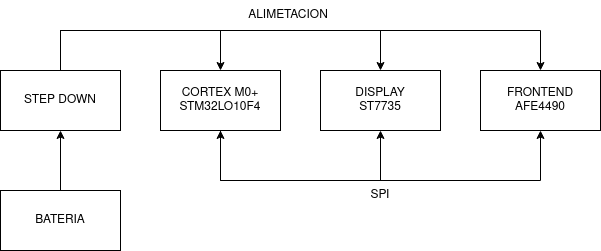
\includegraphics[width=0.8\textwidth]{img/bloques.png}
    \caption{Diagrama en bloques del sistema}
    \label{fig:bloques}
\end{figure}

\begin{figure}[h!]
    \centering
    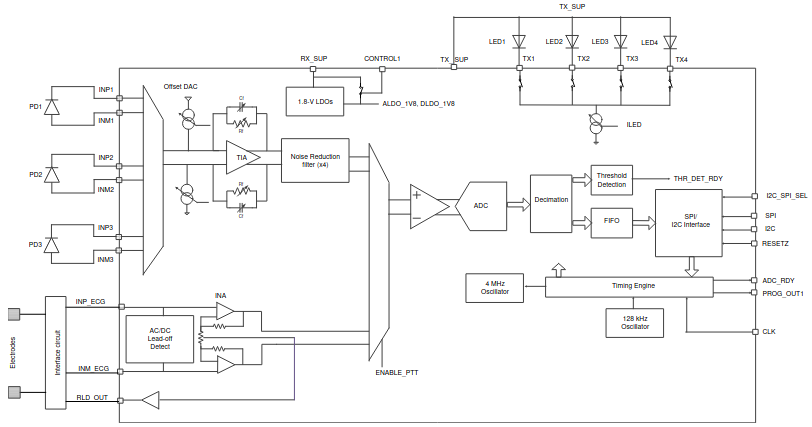
\includegraphics[width=0.8\textwidth]{img/frontend.png}
    \caption{Diagrama en bloques del \emph{frontend}}
    \label{fig:frontend}
\end{figure}

\begin{figure}[h!]
    \centering
    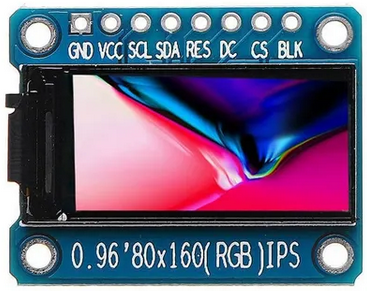
\includegraphics[width=0.4\textwidth]{img/display.png}
    \caption{\emph{Display} a utilizar}
    \label{fig:display}
\end{figure}

\subsection{Normativa aplicable}
\label{subsec:normativa}

El marco normativo aplicable es el siguiente:

\begin{itemize}
    \item Decreto presidencial N° 9763/64 (producción y comercialización de productos médicos)
    \item IEC 60601-2-20 (seguridad eléctrica en equipos médicos)
    \item IEC 62304:2006 (calidad en \emph{software} médico)
    \item ISO 13485:2016 (sistema de gestión de calidad para dispositivos médicos)
    \item Ley 16463/1964 (importación y exportación de productos médicos)
    \item MERCOSUR/GMC/RES N°40/00 (reglamento técnico Mercosur de registro de productos médicos)
    \item Ministerio de Justicia y Derechos Humanos, resolución 41/2001 (Programa Nacional de Garantía de Calidad de la Atención Humana).
\end{itemize}

\section{Conclusión}
\label{suc:conclusion}

Este trabajo permitió familiarizarse con el \emph{frontend} AFE4900 y su principio de funcionamiento.

\end{document}
